\documentclass{beamer}

\usepackage[utf8]{inputenc} 
\usepackage[T1]{fontenc}
\usepackage{lmodern}
\usepackage{graphicx}
\usepackage[english]{babel}

\usepackage{float}
\usepackage{caption}
\usepackage{subcaption}

\usetheme{Frankfurt}

\title[Defense]{PROG1 Project 2}

\author{Simon Bihel}
\institute[ENS Rennes]{
\includegraphics[scale=0.12]{ENS_Rennes.png}\\Computer Science Department, 1st year}
\date{November 6, 2015}

\begin{document}

\section*{Introduction}

	\begin{frame}
		\maketitle
	\end{frame}
	

	
	\begin{frame}
		\frametitle{Summary}
		\tableofcontents
	\end{frame}
	
	\section{Basic version}
	
	\begin{frame}
		\frametitle{Approach}
	\end{frame}

	
	\section{Advanced features}
	\begin{frame}
		\frametitle{Summary}
		\tableofcontents[currentsection]
	\end{frame}

	
	\section*{Conclusion}
	\subsection*{Conclusion}
	\begin{frame}
		\frametitle{Conclusion}
		\begin{block}{Possible improvements}
			\begin{itemize}
				\item making it work;
				\item enhance complexity.
			\end{itemize}
		\end{block}
	\end{frame}
	
	
	\subsection*{Take away}
	\begin{frame}
		\frametitle{~}
		\begin{center}
			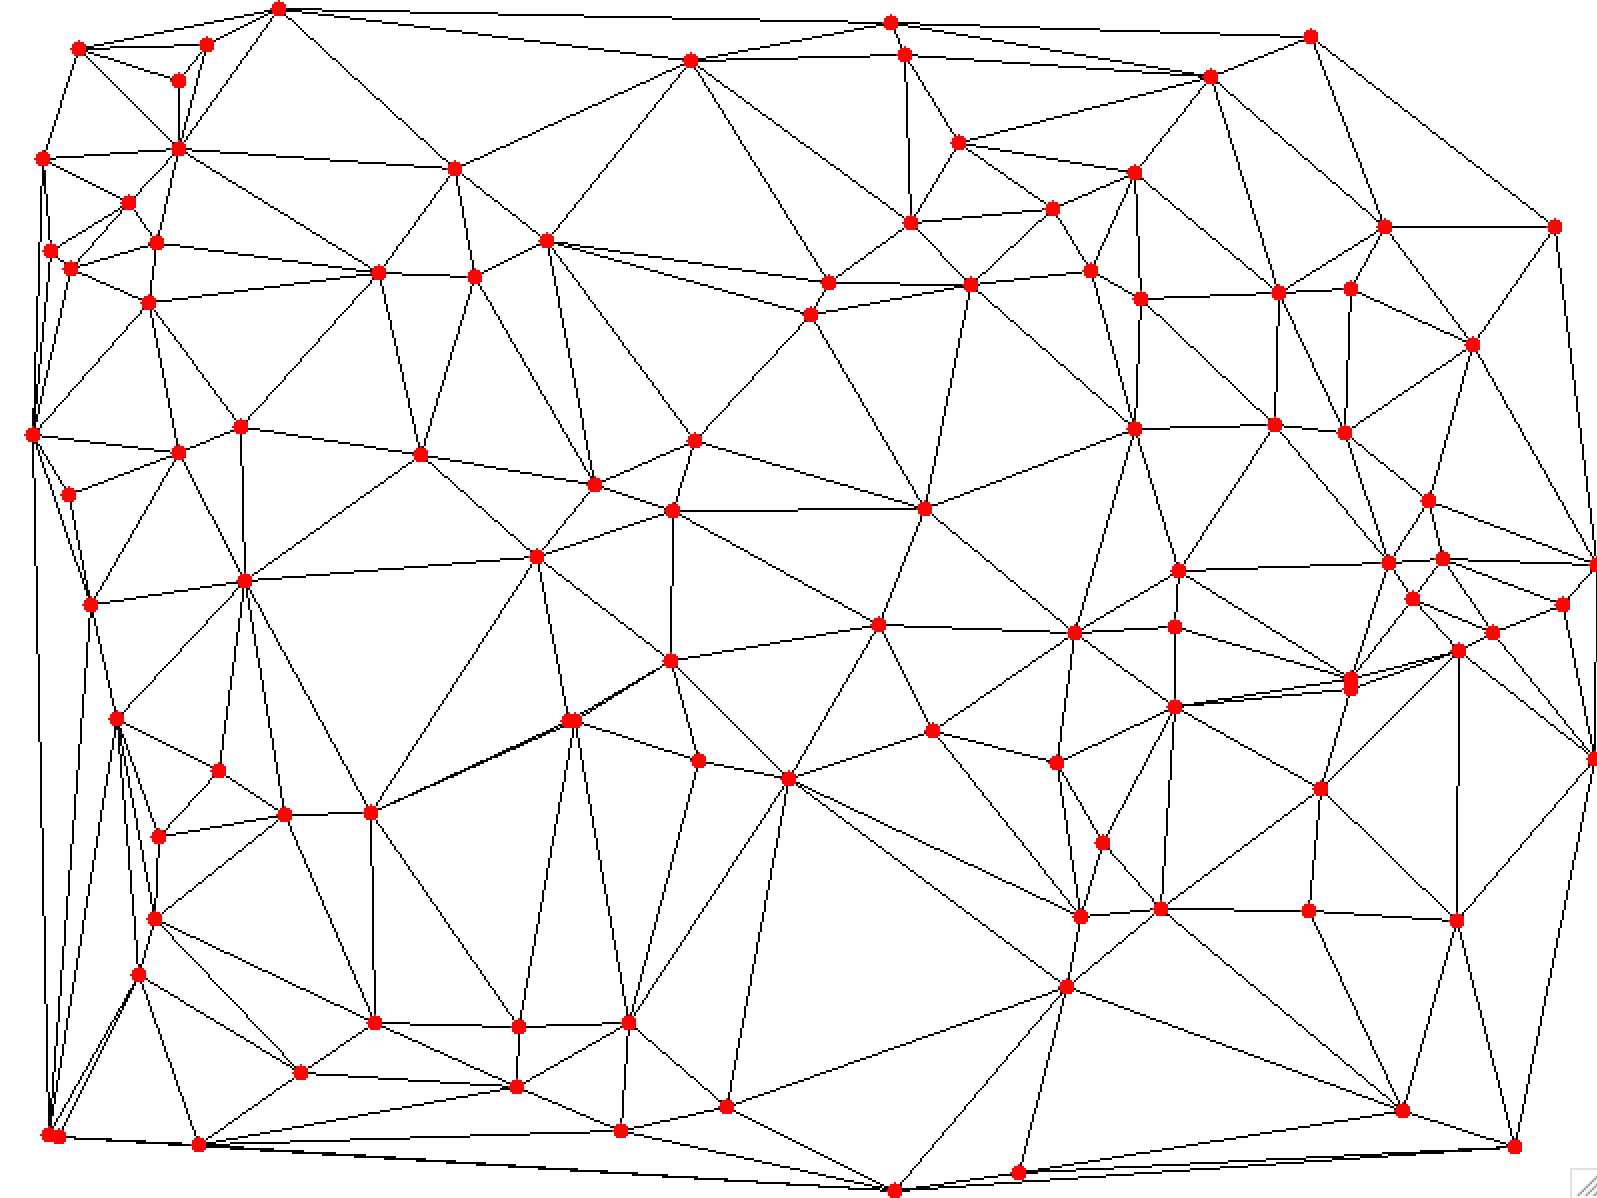
\includegraphics[scale=0.3]{convexhull-good.png}
		\end{center}
	\end{frame}

\end{document}
